\documentclass[tikz,border=10pt]{standalone}
\usetikzlibrary{calc,intersections}

\begin{document}
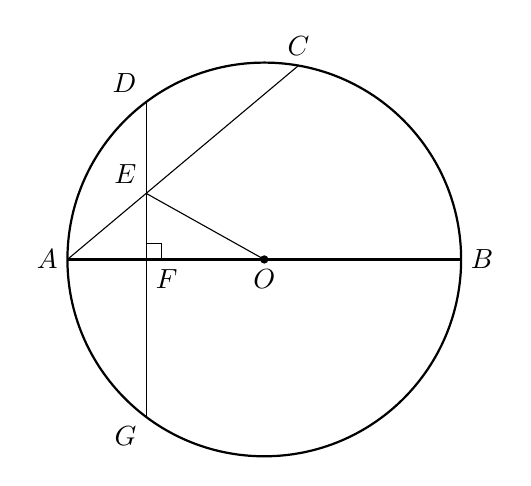
\begin{tikzpicture}
    % 1. 定义圆心和半径
    \coordinate (O) at (0,0);
    \def\r{2.5}
    
    % 2. 绘制圆
    \draw[thick] (O) circle (\r);
    \fill (O) circle (1.5pt) node[below] {$O$};
    
    % 3. 定义直径 AB
    \coordinate (A) at (-\r,0);
    \coordinate (B) at (\r,0);
    \draw[thick] (A) -- (B);
    \node[left] at (A) {$A$};
    \node[right] at (B) {$B$};
    
    % 4. 定义辅助垂直线 DG（修复错误：去掉多余小数点）
    \def\fx{-1.5}  % 错误修复：原代码 \fx{-1.5.2} 非法
    \coordinate (F) at (\fx, 0);
    \node[below right] at (F) {$F$};
    
    % 垂直标记（DF ⊥ AB）
    \draw ($(F)+(0,0.2)$) -- ($(F)+(0.2,0.2)$) -- ($(F)+(0.2,0)$);
    
    % 计算 D、G 坐标（圆上点）
    \pgfmathsetmacro{\fy}{sqrt(\r*\r - \fx*\fx)}
    \coordinate (D) at (\fx, \fy);
    \coordinate (G) at (\fx, -\fy);
    \draw (D) -- (G);
    \node[above left] at (D) {$D$};
    \node[below left] at (G) {$G$};
    
    % 5. 定义点 C
    \coordinate (C) at (80:\r);
    \node[above] at (C) {$C$};
    
    % 6. 求交点 E（AC 与 DG 交点）
    \path[name path=AC] (A) -- (C);
    \path[name path=DG] (D) -- (G);
    \path[name intersections={of=AC and DG, by={E}}];
    
    % 7. 绘制连线
    \draw (A) -- (C);
    \draw (E) -- (O);
    \node[above left] at (E) {$E$};

\end{tikzpicture}
\end{document}